\documentclass{article}
\usepackage{tikz}
\usetikzlibrary{arrows.meta,positioning,calc,shapes.geometric}
\pagestyle{empty}
\begin{document}
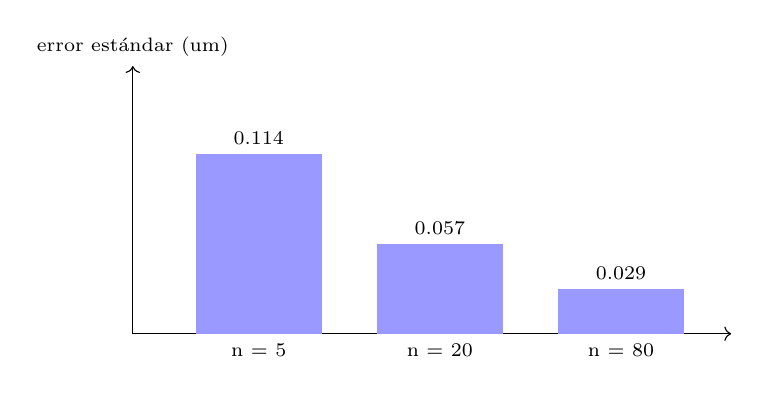
\begin{tikzpicture}
\draw[->] (0,0) -- (0,3.4) node[above, font=\scriptsize] {error estándar (um)}; \draw[->] (0,0) -- (7.6,0);\fill[blue!40] (0.80,0) rectangle (2.40,2.28); \node[font=\scriptsize, above] at (1.60,2.28) {0.114}; \node[font=\scriptsize, below] at (1.60,0) {n = 5};
\fill[blue!40] (3.10,0) rectangle (4.70,1.14); \node[font=\scriptsize, above] at (3.90,1.14) {0.057}; \node[font=\scriptsize, below] at (3.90,0) {n = 20};
\fill[blue!40] (5.40,0) rectangle (7.00,0.57); \node[font=\scriptsize, above] at (6.20,0.57) {0.029}; \node[font=\scriptsize, below] at (6.20,0) {n = 80};

\end{tikzpicture}
\end{document}
